%%%%%%%%%%%%%%%%%%%%%%
% This is an example presentation made with Christopher Gandrud's unofficial LSE Beamer theme
% Updated 27 December 2011
%%%%%%%%%%%%%%%%%%%%%%

\documentclass{beamer}
\usetheme{LSE}
\usepackage{color}
\usepackage{hyperref}
\hypersetup{colorlinks=true,linkcolor=black}
\usepackage{graphics}
\usepackage{tikz}
\usepackage{booktabs}
\usepackage{minted}

%%%%%%%%%%%%%%%%%%%%%%%%%%%%%%%% Title Slide %%%%%%%%%%%%%%%%%%%%%%%%%%
\title[Calcolo Parallelo]{Calcolo Parallelo : Lezione 1}
\author[F. Durastante]{
    \href{mailto:f.durastante@na.iac.cnr.it}{Fabio Durastante}
}
\institute{Consiglio Nazionale delle Ricerche - Istituto per Le Applicazioni del Calcolo ``M. Picone''}
\date[Gennaio 2020]{Master in Scienze e Tecnologie Spaziali, 2020}

\beamerdefaultoverlayspecification{}

\begin{document}

\begin{frame}
	\titlepage
\end{frame}

\section[Outline]{}
\frame{\tableofcontents}

%%%%%%%%%%%%%%%%%%%%%%%%%%%%%%%%%
\section{Scientific and parallel computing}

\begin{frame}{Scientific and parallel computing}

\begin{columns}
	\begin{column}{0.6\textwidth}
		\begin{center}
		``\textbf{Computational science} (also \textbf{scientific computing} or \textbf{scientific computation} (SC)) is a rapidly growing multidisciplinary field that uses advanced computing capabilities to \emph{understand and solve complex problems}. It is an area of science which spans many disciplines, but at its core it involves the development of \emph{models and simulations to understand natural systems}.''
		\end{center}
		
		\flushright Wikipedia
	\end{column}
	\begin{column}{0.4\textwidth}
		\centering
		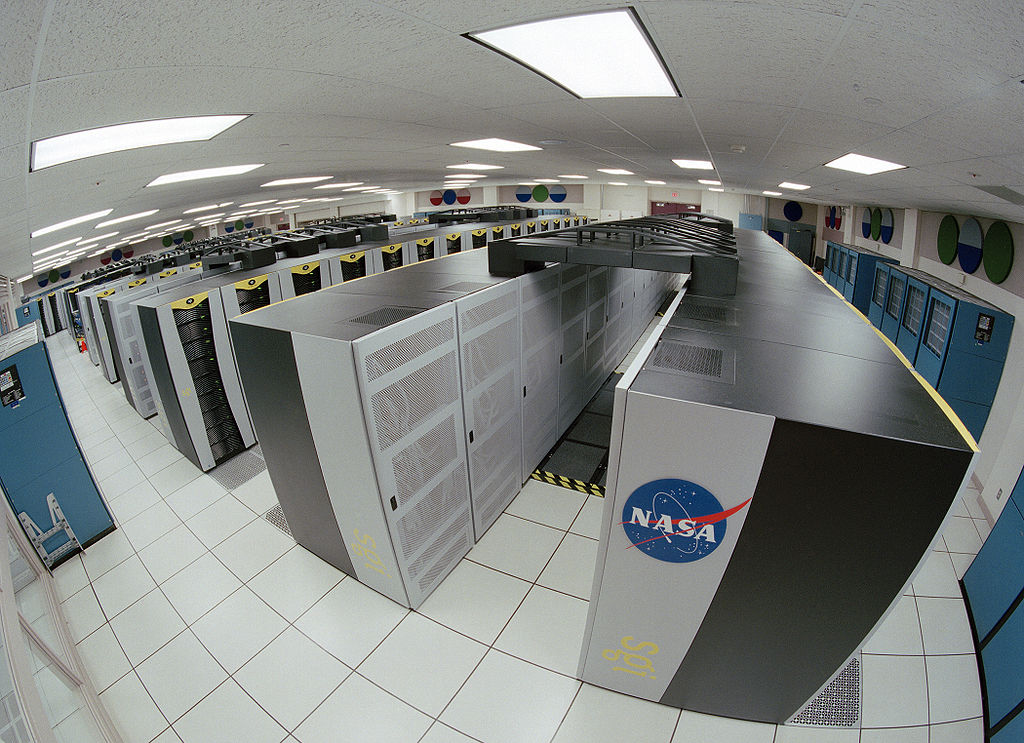
\includegraphics[width=\columnwidth]{nasasuperpc.jpg}
		
	\end{column}
\end{columns}

\end{frame}

\begin{frame}{What are the applications?}
	\centering
	\begin{columns}
		\begin{column}{0.5\textwidth}
		\begin{itemize}
		\item Computational finance,
		\item Computational biology,
		\item Simulation of complex systems,
		\item Network analysis
		\item Multi-physics simulations,
		\item Weather and climate models,
		\item \ldots 
		\end{itemize}
		\end{column}
		\begin{column}{0.5\textwidth}
			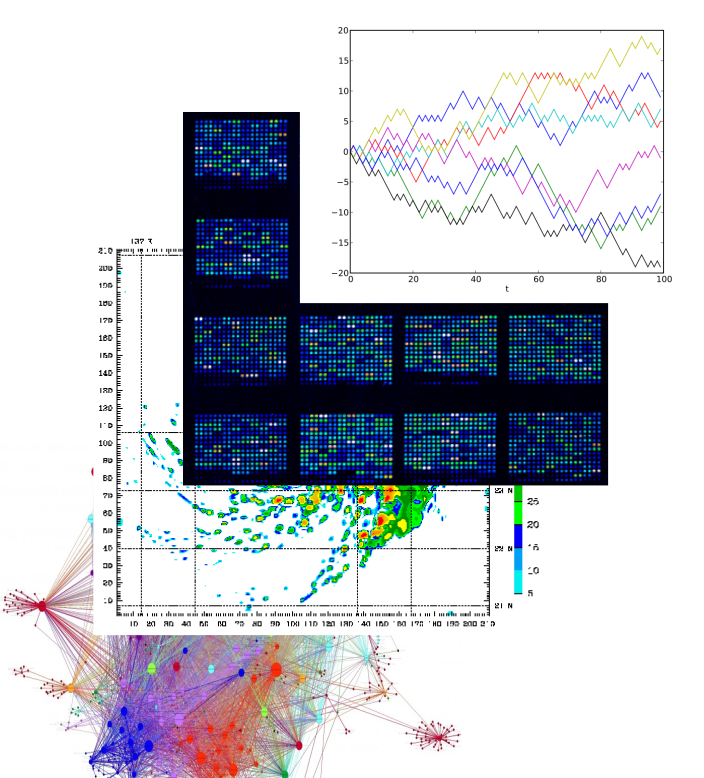
\includegraphics[width=\columnwidth]{applications.png}
		\end{column}
	\end{columns}
	\vfill
	\onslide<2>{Why the need for \alert{parallelism}?}
\end{frame}

\begin{frame}{Moore's law}
	\begin{columns}
		\begin{column}{0.4\columnwidth}
		\centering
		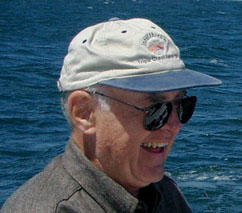
\includegraphics[width=0.3\columnwidth]{Gordon_Moore.jpg}
		
		{\small
			``The complexity for minimum component costs has increased at a rate of roughly a factor of two per year. Certainly over the short term this rate can be expected to continue, if not to increase. Over the longer term, the rate of increase is a bit more uncertain, although there is no reason to believe it will not remain nearly constant for at least 10 years.''
		}
	
		{\flushright G. Moore, 1975}
		\end{column}
	\begin{column}{0.6\columnwidth}
		\centering
		
\includegraphics[width=\columnwidth]{mooreslawoftransistors.png}
		
		\onslide<2>{
		Computers \emph{should} reach the physical limits of Moore's Law at some point in the 2020s\ldots exponential functions saturates physical capabilities!
		}
	\end{column}
	\end{columns}
\end{frame}

\begin{frame}{Motivations for parallel computing}
\begin{itemize}
\item<1-> We are hitting the wall of single processor transistor count/computing capabilities,
\item<2-> Some applications needs more memory than the one that could be available on a single machine,
\item<3-> Optimization of sequential algorithms can bring us only to a certain extent
\end{itemize}
\onslide<4->{
	\centering
	``$\delta\iota\alpha\acute{\iota}\rho\epsilon\iota\,\kappa\alpha\grave{\iota}\,\beta\alpha\sigma\acute{\iota}\lambda\epsilon\nu\epsilon$``\\
	(di\'{a}irei k\'{a}i bas\'{i}leue)}

\onslide<5->{
\centering
Dividi et Impera
}

\onslide<6>{
\flushleft
Therefore, we need
\begin{itemize}
	\item Algorithms that can work in parallel,
	\item A communications protocol for parallel computation integrated with our programming languages
	\item Parallel machines that can actually run this code
\end{itemize}
}
\end{frame}

\subsection{Flynn's Taxonomy}

\begin{frame}{Parallel computers: Flynn's Taxonomy}
Let us start from the bottom: the \alert{machines}.
\begin{itemize}
	\item<2-> What is a parallel computer? \only<3-4>{well, it can be a certain number of different ``things''
	\begin{itemize}
		\item \alert<4>{Multi-core computing}
		\item Symmetric multiprocessing
		\item Distributed computing
		\item \alert<4>{Cluster computing}
		\item \alert<4>{Massively parallel computing}
		\item Grid computing
		\item \alert<4>{General-purpose computing on graphics processing units (GPGPU)}
		\item Vector processors
	\end{itemize}}
	\item<5-> Let us \emph{abstract} from the machine by describing Flynn's taxonomy 
	\begin{columns}
		\begin{column}{0.25\columnwidth}
		\centering
		\small
		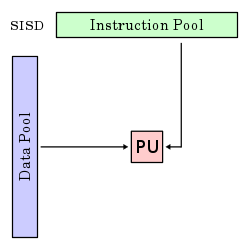
\includegraphics[width=\columnwidth]{SISD.png}
		
		Single instruction stream, single data stream\\SISD
		\end{column}
			\begin{column}{0.25\columnwidth}
						\centering
				\small
	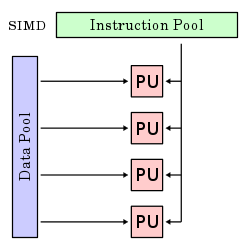
\includegraphics[width=\columnwidth]{SIMD.png}
	
	\alert<6>{Single instruction stream, multiple data streams\\SIMD}
	\end{column}
		\begin{column}{0.25\columnwidth}
					\centering
			\small
	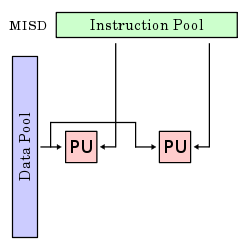
\includegraphics[width=\columnwidth]{MISD.png}
			
	Multiple instruction streams, single data stream\\MISD
\end{column}
\begin{column}{0.25\columnwidth}
					\centering
			\small
	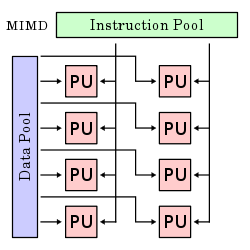
\includegraphics[width=\columnwidth]{MIMD.png}			
	
	\alert<6->{Multiple instruction streams, multiple data streams\\MIMD}
\end{column}
	\end{columns}
\end{itemize}
\end{frame}

\begin{frame}{Parallel Computers: our computer model}
For our task of introducing parallel computations we need to fix a \textbf{specific multiprocessor model}, i.e., a specific generalization of the sequential RAM model in which there is more than one processor.
\vfill
\begin{columns}
	\begin{column}{0.5\columnwidth}
	Since we want to stay in a SIMD/MIMD model, we focus on a \emph{local memory machine model}, i.e., a set of $M$ processors each with its own local memory that are attached to a common communication network.
	\end{column}
	\begin{column}{0.5\columnwidth}
	\centering
	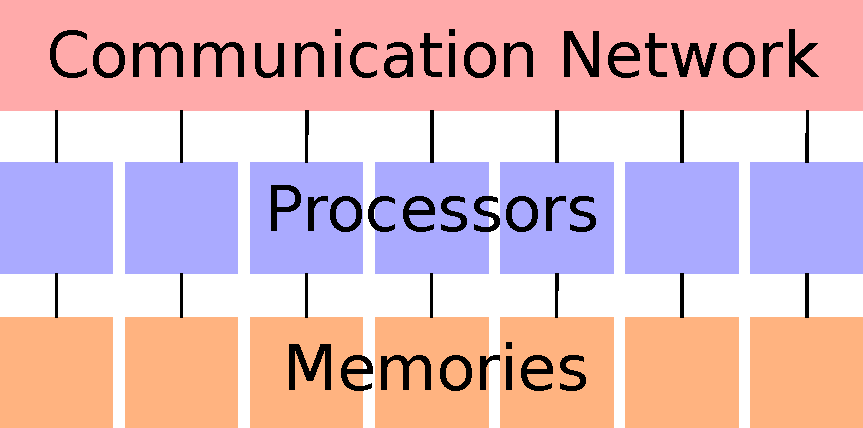
\includegraphics[width=\columnwidth]{networkarchitecture.pdf}
	\end{column}
\end{columns}
\vfill
\only<2>{
\begin{itemize}
	\item We can be more precise about the connection between processors, one can consider a network (a collection of switches connected by communication channels) and delve in a detailed way into its pattern of interconnection, i.e., into what is called the network topology.
\end{itemize}
}
\only<3>{
\begin{itemize}
	\item An alternative is to summarize the network properties in terms of two parameters: \alert{latency} and \alert{bandwidth}
	\begin{description}
		\item[Latency] the time it takes for a message to traverse the network;
		\item[Bandwidth] the rate at which a processor can inject data into the network.
	\end{description}
\end{itemize}
}


%\vfill
%\onslide<3>{
%	\centering
%	What are the available machines?
%}
\end{frame}


\subsection{The TOP500 List}

\begin{frame}{The TOP500 List -- \url{https://www.top500.org/}}
\begin{columns}
	\begin{column}{0.4\columnwidth}
	\small
	``\ldots we have decided in 1993 to assemble and maintain a list of the 500 most powerful computer systems. Our list has been compiled twice a year since June 1993 with the help of high-performance computer experts, computational scientists, manufacturers, and the Internet community in general\ldots
	
	In the present list (which we call the TOP500), we list computers ranked by their performance on the \alert{LINPACK Benchmark}.''
	\vfill
	\url{http://www.netlib.org/benchmark/hpl/}
	\end{column}
	\begin{column}{0.6\textwidth}
	\small
	\onslide<2>{
	The \alert{LINPACK} Benchmark.
	
	Solution of a dense $n\times n$  system of linear equations $A\mathbf{x} = \mathbf{b}$, so that
	\begin{itemize}
		\item $\frac{\| A \mathbf{x} - \mathbf{b}\|}{\|A\|\|\mathbf{x}\| n \varepsilon} \leq O(1)$, for $\varepsilon$ machine precision,
		\item It uses a specialized right--looking LU factorization with look--ahead
		\item Measuring 
		\begin{itemize}
			\item $R_\text{max}$ the performance in GFLOPS for the largest problem run on a machine,
			\item $N_\text{max}$ the size of the largest problem run on a machine,
			\item $N_{1/2}$ the size where half the $R_\text{max}$ execution rate is achieved,
			\item $R_{\text{peak}}$ the theoretical peak performance GFLOPS for the machine.
		\end{itemize}
	\end{itemize}
	
	

	}
	\end{column}
\end{columns}
\end{frame}


\section{Parallel Algorithms}

\begin{frame}{Parallel Algorithms}
In a fairly general way we can say that a \textbf{parallel algorithm} is an algorithm which can do \emph{multiple operations} in a given time.

\onslide<2->{\textbf{Example:} the sum of two vectors $\mathbf{x}, \mathbf{y} \in \mathbb{R}^n$

\begin{equation*}
	\begin{array}{cl}
	\mathbf{x} & = [x_1 \; x_2 \; \cdots \; x_i  \;\onslide<3>{\textcolor{blue}{\boldsymbol{|}}\;} x_{i+1} \; \cdots x_n] \\
	+ \\
	\mathbf{y} & = [y_1 \; y_2 \; \cdots \; y_i  \;\onslide<3>{\textcolor{blue}{\boldsymbol{|}}\;} y_{i+1} \; \cdots y_n] \\
	= \\
	\mathbf{x} + \mathbf{y} & = [x_1+y_1 \; x_2+y_2 \; \cdots \; x_i+y_i  \;\onslide<3>{\textcolor{blue}{\boldsymbol{|}}\;} \cdots x_n+y_n] \\
	\end{array}
\end{equation*}
\begin{itemize}
	\item<2-> If we do the operation sequentially we do $O(n)$ operations in $T_n$
	\item<3-> If we split the operation among $2$ processors, one summing up the entries between $1,\ldots,i$, and one summing up the entries between $i+1,\ldots,n$ we take $T_i$ time for the first part and $T_{n-i}$ time for the second, therefore the overall time is $\max(T_{i},T_{n-i})$ for doing always $O(n)$ operations.
\end{itemize}

}
\end{frame}

\begin{frame}{Parallel Algorithms: \emph{speedup}}
\small
Let us try to think again in an abstract way and to quantify the \alert{overall speed gain} for a given gain in a subset of a process.
\begin{itemize}
	\item<1-> We break some process into $N$ distinct portions with the $i$th portion occupying the $P_i$ fraction of the overall completion time,
	\item<2-> then we order such portion in such a way that the $N$th portions subsumes all the parts of the overall processes that have fixed costs.
	\item<3-> The \emph{speedup} of the $i$th portion can then be defined as 
	\begin{equation*}
		S_i \triangleq \frac{t_{\text{original}}}{t_{\text{optimized}}}, \quad i=1,\ldots,N-1
	\end{equation*}
	where the numerator and denominator are the original and optimized completion time.
%	\item<4-> 
\end{itemize}
\begin{block}<4>{Amdahl's Law}
Then the \textcolor{blue}{overall speedup} for $\mathbf{P} = (P_1,\ldots,P_N)$, $\mathbf{S} = (S_1,\ldots,S_{N-1})$ is:
\begin{equation*}
S(\mathbf{P},\mathbf{S}) = \left(P_N + \sum_{i=1}^{N-1} \frac{P_i}{S_i}\right)^{-1}.
\end{equation*}
\end{block}

\end{frame}

\begin{frame}{Parallel Algorithms: \emph{Amdahl's Law}}
Let us make some observations on Amdahl's Law
\begin{itemize}
	\item We are not assuming about whether the original completion time  involves some optimization,
	\item We are not making any assumption on what our optimization process is,
	\item We are not even saying that the process in question involves a computer!
\end{itemize}
Amdahl's Law is a fairly general way of looking at how processes can be speed up by dividing them into sub-tasks with lower execution time. 

\onslide<2>{Moreover, it fixes  the \alert{theoretical maximum speedup} in various scenarios.
\begin{itemize}
	\item If we allow all components $S_i$ to grow unbounded then the upper bound on all scenario si $S_{\text{max}} = 1/P_N$.
\end{itemize}
Let us decline it in the context of the potential utility of \emph{parallel hardware}.
}
\end{frame}

\begin{frame}{Parallel Algorithms: \emph{Amdahl's Law} for \emph{parallel hardware}}
 Consider now having a parallel machine that permits us dividing the execution of code across $M$ hardware units, then the problem independent maximum speedup that such hardware can provide is $M$.
 \begin{block}{Parallel Efficiency}
 We define the parallel efficiency $E$ as
 \begin{equation*}
 	E \triangleq \frac{S_{\text{overall}}}{M},
 \end{equation*}
 where $E = 100\%$ correspond to the maximal use of the available hardware. When $S_{\text{max}} < M$, it is then impossible to take full advantage of all available execution units.
 \end{block}
\onslide<2->{\alert{Goal:} we require very large $S_{\text{max}}$ and correspondingly tiny $P_N$.}

\onslide<3->{\begin{center}
	\underline{Every dusty corner of a code must scale}, any portion that doesn't becomes the rate-limiting step!
\end{center}}
 
\end{frame}

\begin{frame}{Parallel Algorithms: \emph{Amdahl's Law} limitations}
What we are neglecting and what we are tacitly assuming
\begin{itemize}
	\item We are neglecting \emph{overhead costs}, i.e., the cost associated with parallel execution such as
	\begin{itemize}
		\item initializing (spawning) and joining of different computation threads,
		\item communication between processes, data movement and memory allocation.
	\end{itemize}
	\item We considered also the ideal case in which $S_i \rightarrow +\infty$ $\forall i$, observe that with finite speedup on portions $1$ through $N-1$, the $S_{\text{overall}}$ might continue to improve with increasing number of execution units.
	\item We are assuming that the size of the problem remains fixed while the number of execution units increases, this is called the case of \alert{strong scalability}. In some contexts, we need to turn instead to \alert{weak scalability} in which the problem size grows proportionally to the number of execution units.
\end{itemize}
\end{frame}

\section{Message Passing Interface}

\begin{frame}{How do we realize practically this parallelism?}
Let us focus on what we have discussed until now:
\begin{itemize}
	\item We have ``machines'' with multiple processors and whose main memory is partitioned into fragmented components,
	\item We have algorithms that can divide a problem of size $N$ among these processors so that they can run (almost) independently,
	\item With a certain degree of approximation, we know how to compute what is the \emph{best improvement} we can expect from a parallel program with $M$ processors on a problem of size $N$.
\end{itemize}
What we need to discuss now is then: ``How can we actually implement these algorithms on real machines?''
\begin{itemize}
	\item We need a way to define a parallel environment in which every processor is accounted for,
	\item We need to have data formats that are aware of the fact that we have a \emph{distributed} memory,
	\item We need to exchange data between the various memory fragments.
\end{itemize}
\end{frame}

\begin{frame}{Message Passing Interface -- \url{https://www.mpi-forum.org/}}

\begin{quote}
	``MPI (Message Passing Interface) is a \alert{specification for a standard library} for message passing that was defined by the MPI Forum, a broadly based group of parallel computer vendors, library writers, and applications specialists.'' -- W. Gropp, E. Lusk, N. Doss, A. Skjellum,
	\emph{A high-performance, portable implementation of the MPI message passing interface standard}, Parallel Computing, 22 (6), 1996.
\end{quote}

\begin{itemize}
	\item<2-> MPI implementations consist of a specific set of routines directly callable from C, C++, Fortran;
	\item<3-> MPI uses Language Independent Specifications for calls and language bindings;
	\item<4-> The MPI interface provides an essential \emph{virtual} topology, synchronization, and communication functionality inside a set of processes.
	\item<5-> There exist many implementations of the MPI specification, e.g., MPICH, Open MPI, pyMPI
\end{itemize}
\end{frame}

\subsection{Our First MPI Program}

\begin{frame}[fragile]{Hello (parallel) world!}
In all the course we are going to use the MPI inside C programs.
\begin{columns}
\begin{column}{0.4\columnwidth}
\begin{minted}{c}
#include"mpi.h"
#include<stdio.h>

int main(int argc, 
	char **argv){
 MPI_Init( &argc, &argv);
 printf("Hello, world!\n");
 MPI_Finalize();
 return 0;
}
\end{minted}
\end{column}
\begin{column}{0.56\columnwidth}
\small
\begin{itemize}
	\item \mintinline{c}{#include "mpi.h"} provides basic MPI definitions and types,
	\item \mintinline{c}{MPI_Init} start MPI, it has to precede any MPI call!
	\item \mintinline{c}{MPI_Finalize} exits MPI
	\item All the non--MPI routines are local!
\end{itemize}
\end{column}
\end{columns}
\vfill
\onslide<2>{We need now to \emph{compile} and \emph{link} the \mintinline{bash}{helloworld.c} program, and we can do it simply by:
\
\mint{bash}{mpicc helloworld.c -o helloworld}
}
\end{frame}

\begin{frame}[fragile]{Hello (parallel) world! -- Compile, Link and Run}
\mint{bash}{mpicc helloworld.c -o helloworld}
\begin{itemize}
	\item \mintinline{bash}{mpicc} is a wrapper for a C compiler provided by the Open MPI implementation of MPI.
	\item the option \mintinline{bash}{-o} sets the name of the compiled (executable) file.
\end{itemize}
\onslide<2->{Let us see what is happening behind the curtains}
\begin{itemize}
	\item<2-> you can first try to discover what compiler are you using by executing \mintinline{bash}{mpicc --version}, \begin{onlyenv}<2>
that will give you something like
\begin{minted}{bash}
icc (ICC) 17.0.4 20170411
Copyright (C) 1985-2017 Intel Corporation.  
All rights reserved.
\end{minted} 
for an Intel compiler, or maybe
\begin{minted}{bash}
gcc (Ubuntu 7.4.0-1ubuntu1~18.04.1) 7.4.0
Copyright (C) 2017 Free Software Foundation, Inc.
\end{minted}		
	\end{onlyenv}
\item<3-> or discover what are the library inclusion and linking options by asking for \mintinline{bash}{mpicc --showme:compile} and \mintinline{bash}{mpicc --showme:link}, respectively.
\item<4-> In general, looking at the output of the \mintinline{bash}{man mpicc} command is always a good idea.
\end{itemize} 
\only<5>{{\centering\small``If you find yourself saying, "But I don't want to use wrapper compilers!", please humor us and try them. See if they work for you. Be sure to let us know if they do not work for you. '' - {\scriptsize \url{https://www.open-mpi.org/faq/?category=mpi-apps}}}}
\end{frame}

\begin{frame}[fragile]{Hello (parallel) world! -- Compile, Link and Run}
A piece of advice: if your program is anything more realistic than a classroom exercise use \mintinline{bash}{make}\footnote{\url{https://www.gnu.org/software/make/}}, and save yourself from writing painfully long compiling commands, and dealing with complex dependencies more than once.

\begin{quote}
``Make gets its knowledge of how to build your program from a file called the makefile, which lists each of the non-source files and how to compute it from other files.''
\end{quote}

A very simple \mintinline{bash}{Makefile} for our first test would be
\begin{minted}{Makefile}
MPICC = mpicc #The wrapper for the compiler
CFLAGS += -g  #Useful for debug symbols
all: helloworld
helloworld: helloworld.c
  $(MPICC) $(CFLAGS) $(LDFLAGS) $? $(LDLIBS) -o $@
clean:
  rm -f helloworld
\end{minted}
\end{frame}

\begin{frame}[fragile]{Hello (parallel) world! -- Compile, Link and Run}
Let us run our first parallel program by doing:
\mint{bash}{mpirun [ -np X ] [ --hostfile <filename> ]  helloworld}
or by using its synonym
\mint{bash}{mpiexec [ -np X ] [ --hostfile <filename> ]  helloworld}
\begin{itemize}
	\item<1-> \mintinline{bash}{mpirun}/\mintinline{bash}{mpiexec} will  run  \mintinline{bash}{X} copies of \mintinline{bash}{helloworld} in your current run-time environment, scheduling (by default) in a round-robin fashion by CPU slot.
	\item<1-> if running under a supported resource manager, Open MPI's \mintinline{bash}{mpirun} will usually automatically use the corresponding resource manager process starter, as opposed to, for example, rsh or ssh, which require the use of a hostfile, or will default  to  running all \mintinline{bash}{X} copies on the localhost 
	\item<2-> as always, look at the manual, by doing \mintinline{bash}{man mpirun}.
\end{itemize}

\end{frame}


\begin{frame}[fragile]{Hello (parallel) world! -- Compile, Link and Run}
If we now run
\mint{bash}{mpirun -np 6 helloworld}
we get the following output:
\begin{columns}
\begin{column}{0.4\columnwidth}
\begin{minted}{bash}
Hello, world!
Hello, world!
Hello, world!
Hello, world!
Hello, world!
Hello, world!
\end{minted}
\end{column}
\begin{column}{0.6\columnwidth}
Every process executes the line \mint{c}{printf("Hello, world!\n");} that it is a \alert{local} routine!
\end{column}
\end{columns}
\begin{block}<2>{local vs non-local procedure}
	A procedure is \textbf{local} if completion of the procedure depends only on the local executing process.
	
	A procedure is \textbf{non-local} if completion of the operation may require the execution of some MPI procedure on another process. Such an operation \emph{may require
	communication} occurring with another user process.
\end{block}
\end{frame}

\subsection{The MPI parallel environment}
\begin{frame}[fragile]{The MPI parallel environment}
Let us modify our \mintinline{bash}{helloworld} to investigate the MPI parallel environment. Specifically, we want to answer, from within the program, to the questions:
\begin{enumerate} 
	\item How many processes are there?
	\item Who am I?
\end{enumerate}
\begin{minted}{c}
#include "mpi.h"
#include <stdio.h>
int main( int argc, char **argv ){
 int rank, size;
 MPI_Init( &argc, &argv );
 MPI_Comm_rank( MPI_COMM_WORLD, &rank );
 MPI_Comm_size( MPI_COMM_WORLD, &size );
 printf( "Hello world! I'm process %d of %d\n",rank, size );
 MPI_Finalize();
 return 0;
}
\end{minted}
\end{frame}

\begin{frame}[fragile]{The MPI parallel environment}
\begin{minted}{c}
#include "mpi.h"
#include <stdio.h>
int main( int argc, char **argv ){
 int rank, size;
 MPI_Init( &argc, &argv );
 MPI_Comm_rank( MPI_COMM_WORLD, &rank );
 MPI_Comm_size( MPI_COMM_WORLD, &size );
 printf( "Hello world! I'm process %d of %d\n",rank, size );
 MPI_Finalize();
 return 0;
}
\end{minted}
\begin{itemize}
	\item How many is answered by a call to \mintinline{c}{MPI_Comm_size} as an \mintinline{c}{int} value,
	\item Who am I? Is answered by a call to \mintinline{c}{MPI_Comm_rank} as an \mintinline{c}{int} value that is conventionally called \mintinline{c}{rank} and is a number between \mintinline{c}{0} and \mintinline{c}{size-1}.
\end{itemize}
\end{frame}


\begin{frame}{The MPI parallel environment}
	The last keyword we need to describe is the \mintinline{c}{MPI_COMM_WORLD}, this is the standard Communicator object.

	\begin{block}{Communicator}
	A Communicator object connects a group of processes in one MPI session. There can be more than one communicator in an MPI session, each of them gives each contained process an independent identifier and arranges its contained processes in an ordered topology.
	\end{block}

	This provides
	\begin{itemize}
	\item a safe communication space, that guarantees that the code can communicate as they
	need to, without conflicting with communication extraneous to the present code, e.g., if other parallel libraries are in use,
	\item a unified object for conveniently denoting communication context, the group of communicating processes and to house abstract process naming.
	\end{itemize}
\end{frame}

\begin{frame}[fragile]{The MPI parallel environment}
If we have saved our inquiring MPI program in the file \mintinline{bash}{hamlet.c}, we can then modify our \mintinline{bash}{Makefile} by modifying/adding the lines
\begin{minted}{Makefile}
all: helloworld hamlet
hamlet: hamlet.c
 $(MPICC) $(CFLAGS) $(LDFLAGS) $? $(LDLIBS) -o $@
clean:
 rm -f helloworld hamlet
\end{minted}
Then, we compile everything by doing \mintinline{bash}{make hamlet} (or, simply, \mintinline{bash}{make}).

\begin{onlyenv}<2->
When we run the code with \mintinline{bash}{mpirun -np 6 hamlet} we see
\begin{columns}
\begin{column}{0.5\columnwidth}
\begin{verbatim}
Hello world! I'm process 1 of 6
Hello world! I'm process 5 of 6
Hello world! I'm process 0 of 6
Hello world! I'm process 3 of 6
Hello world! I'm process 2 of 6
Hello world! I'm process 4 of 6
\end{verbatim}
\end{column}
\begin{column}{0.5\columnwidth}
\begin{itemize}
	\item<3-> Every processor answers the call,
	\item<4-> But it answers it as soon as he has done doing the computation! There is \alert{no synchronization}.
\end{itemize}
\end{column}
\end{columns}
\end{onlyenv}
\end{frame}

\subsection{When to travek the MPI road}
\begin{frame}{A word of advice}
When should you \textbf{not} write parallel code with MPI?
\begin{itemize}
	\item<1-> The effort of writing optimized and scalable MPI codes is not negligible, therefore a direct usage of it its usually best suited for developing \emph{libraries for scientific computations}. 
	\item<2-> If there is a library containing a good (possibly open source) parallel implementation of the algorithm and the data structure you need: LEARN IT AND USE IT!
\end{itemize}
When should you write parallel code with MPI?
\begin{itemize}
	\item<3-> When you are learning about parallel computing with distributed memory!
	\item<4-> To \emph{really} understand what the instructions manuals of such parallel libraries are telling you,
	\item<5-> Sometimes it happens, you are using a library based on MPI and some function that you truly need is not included. 
	\item<6-> To develop new and better libraries for your scientific challenge!
\end{itemize}
\end{frame}

\section{References}

\begin{frame}{References}
There are more books, notes, tutorials, online courses and oral tradition on scientific and parallel computing than we would have time to read and listen in a life. Pretty much everything that contains the words Parallel Programming and Scientific Computing is good\ldots 

I suggest here the book
\begin{thebibliography}{10}
	\bibitem{rouson} Rouson, D., Xia, J., \& Xu, X. (2011). Scientific software design: the object-oriented way. Cambridge University Press.
\end{thebibliography}
that discusses general aspect of scientific computing (not perfectly related to parallel computing), and to have on your bedside
\begin{thebibliography}{10}
	\bibitem{mpimanual}  Message Passing Interface Forum. MPI: A Message-Passing Interface Standard, Version 3.1. \url{https://www.mpi-forum.org/docs/mpi-3.1/mpi31-report.pdf}, High Performance Computing Center Stuttgart (HLRS).
\end{thebibliography}
\end{frame}


%\begin{frame}{Una storia che viene da lontano$\ldots$}
%\begin{columns}
%\begin{column}{0.20\textwidth}
%	\centering
%	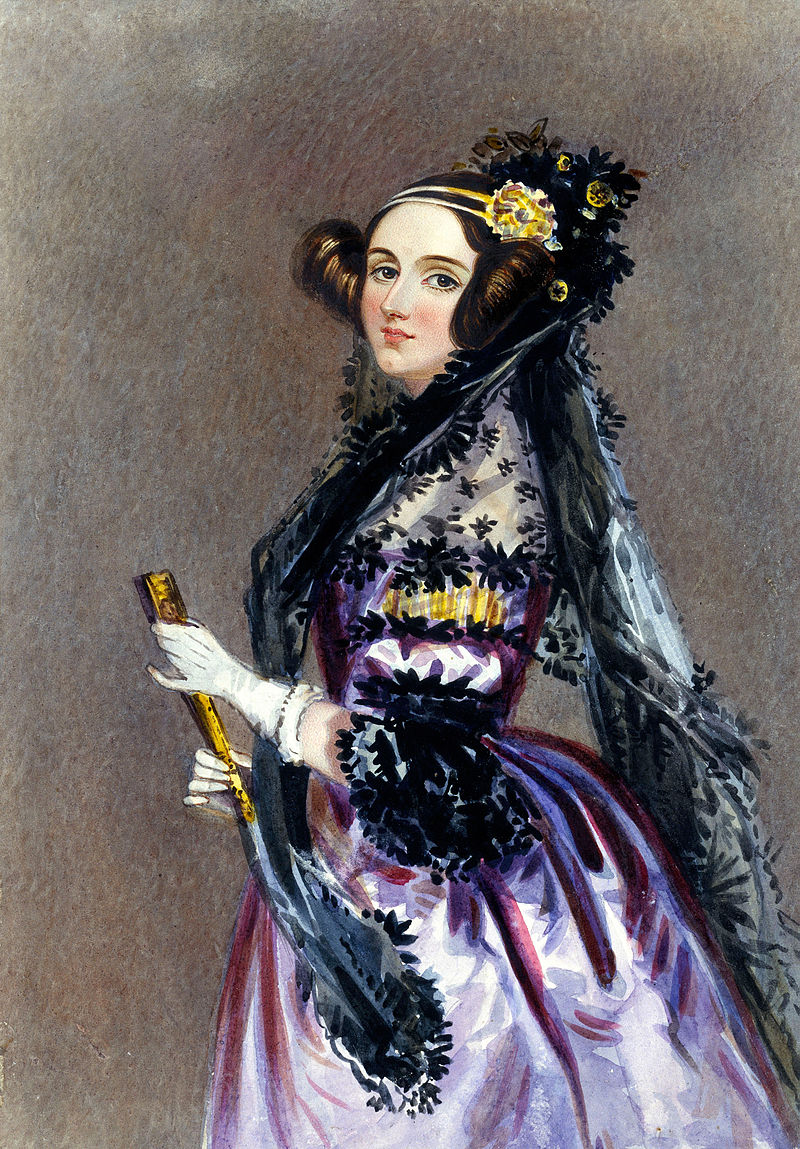
\includegraphics[width=\columnwidth]{AdaLovelace.jpg}
%	
%	\onslide<2->{Ada Lovelace}
%\end{column}
%\begin{column}{0.20\textwidth}
%	\centering
%	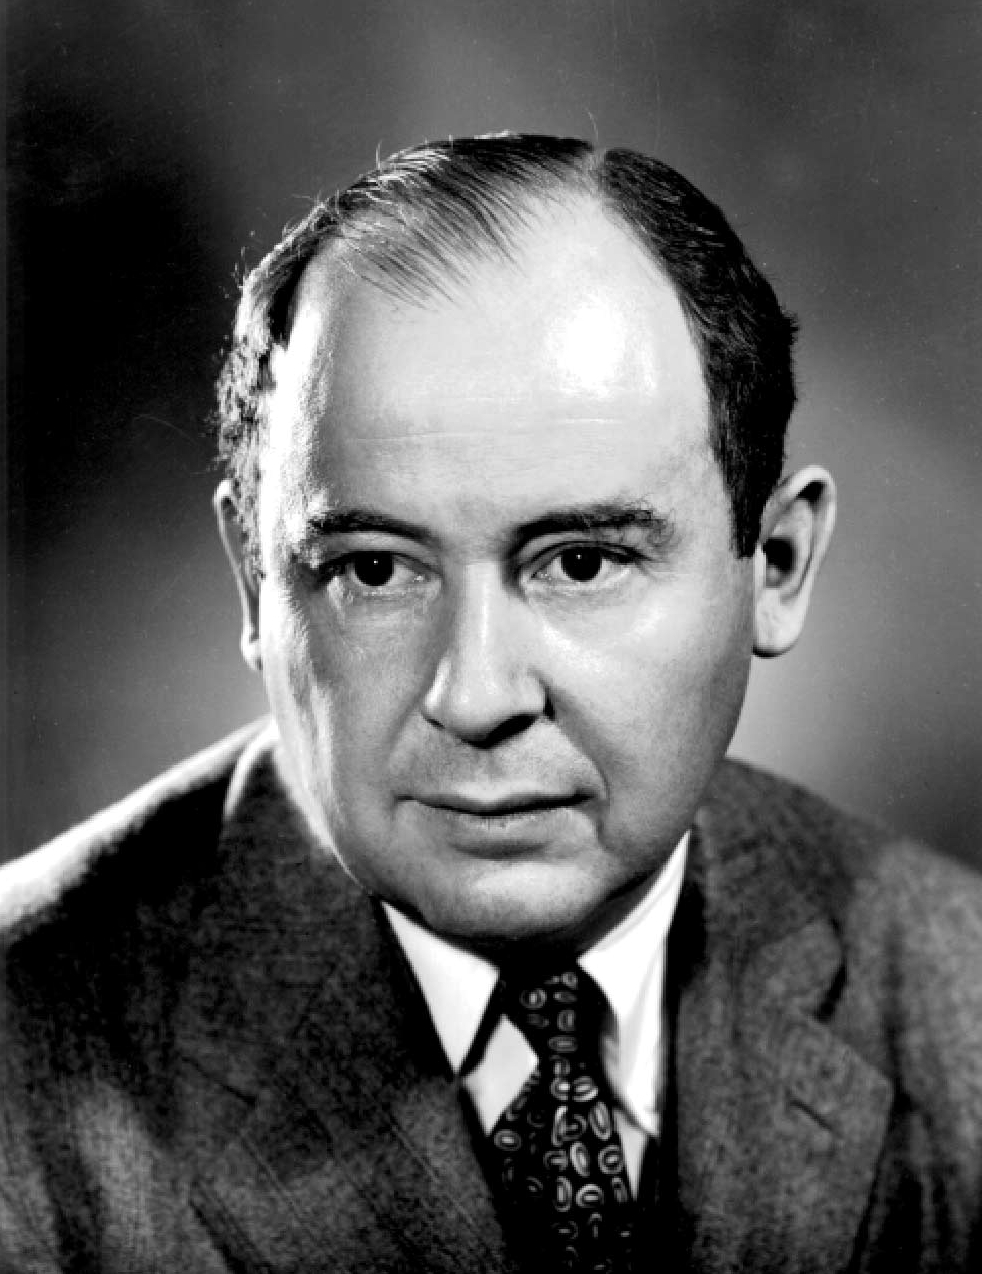
\includegraphics[width=\columnwidth]{JohnvonNeumann.jpg}
%	
%	\onslide<3->{John von Neumann}
%\end{column}
%\begin{column}{0.20\textwidth}
%	\centering
%	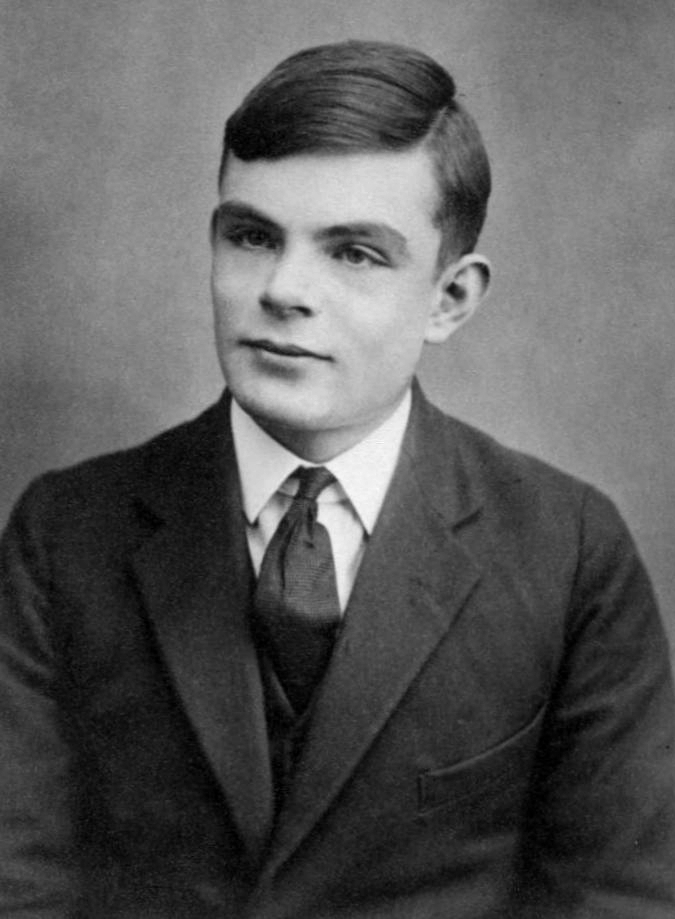
\includegraphics[width=\columnwidth]{AlanTuring.jpg}
%	
%	\onslide<4->{Alan Turing}
%\end{column}
%\begin{column}{0.20\textwidth}
%	\centering
%	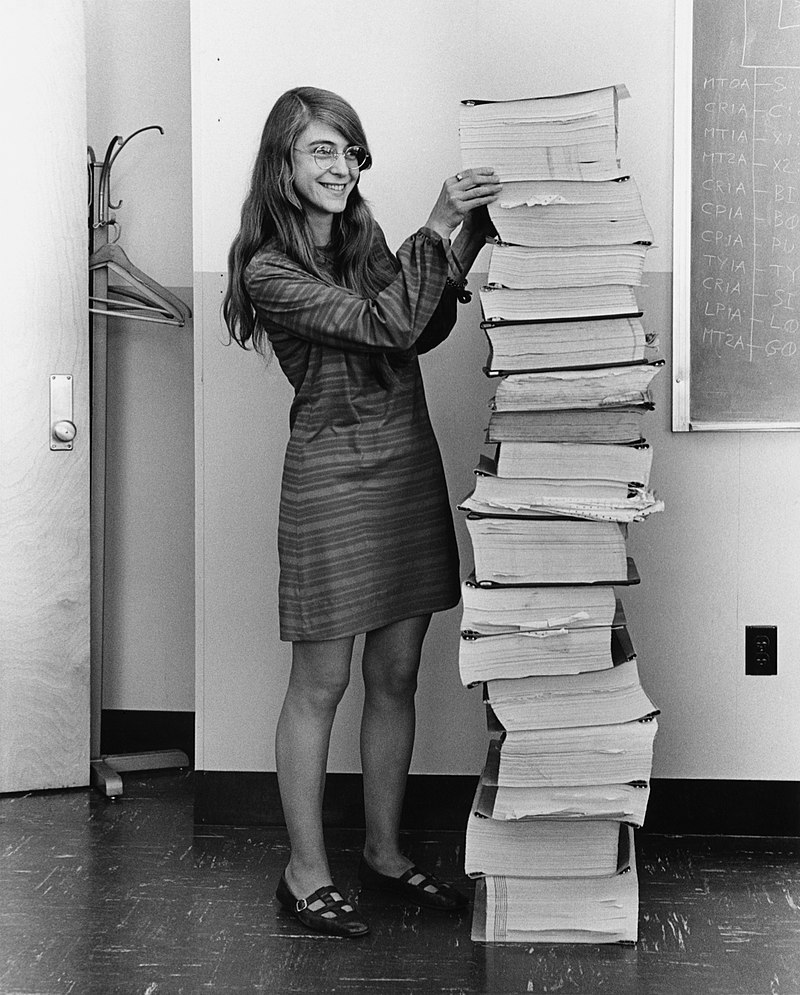
\includegraphics[width=\columnwidth]{MargaretHamilton.jpg}
%	
%	\onslide<5->{Margaret Hamilton}
%\end{column}
%\begin{column}{0.20\textwidth}
%	\centering
%	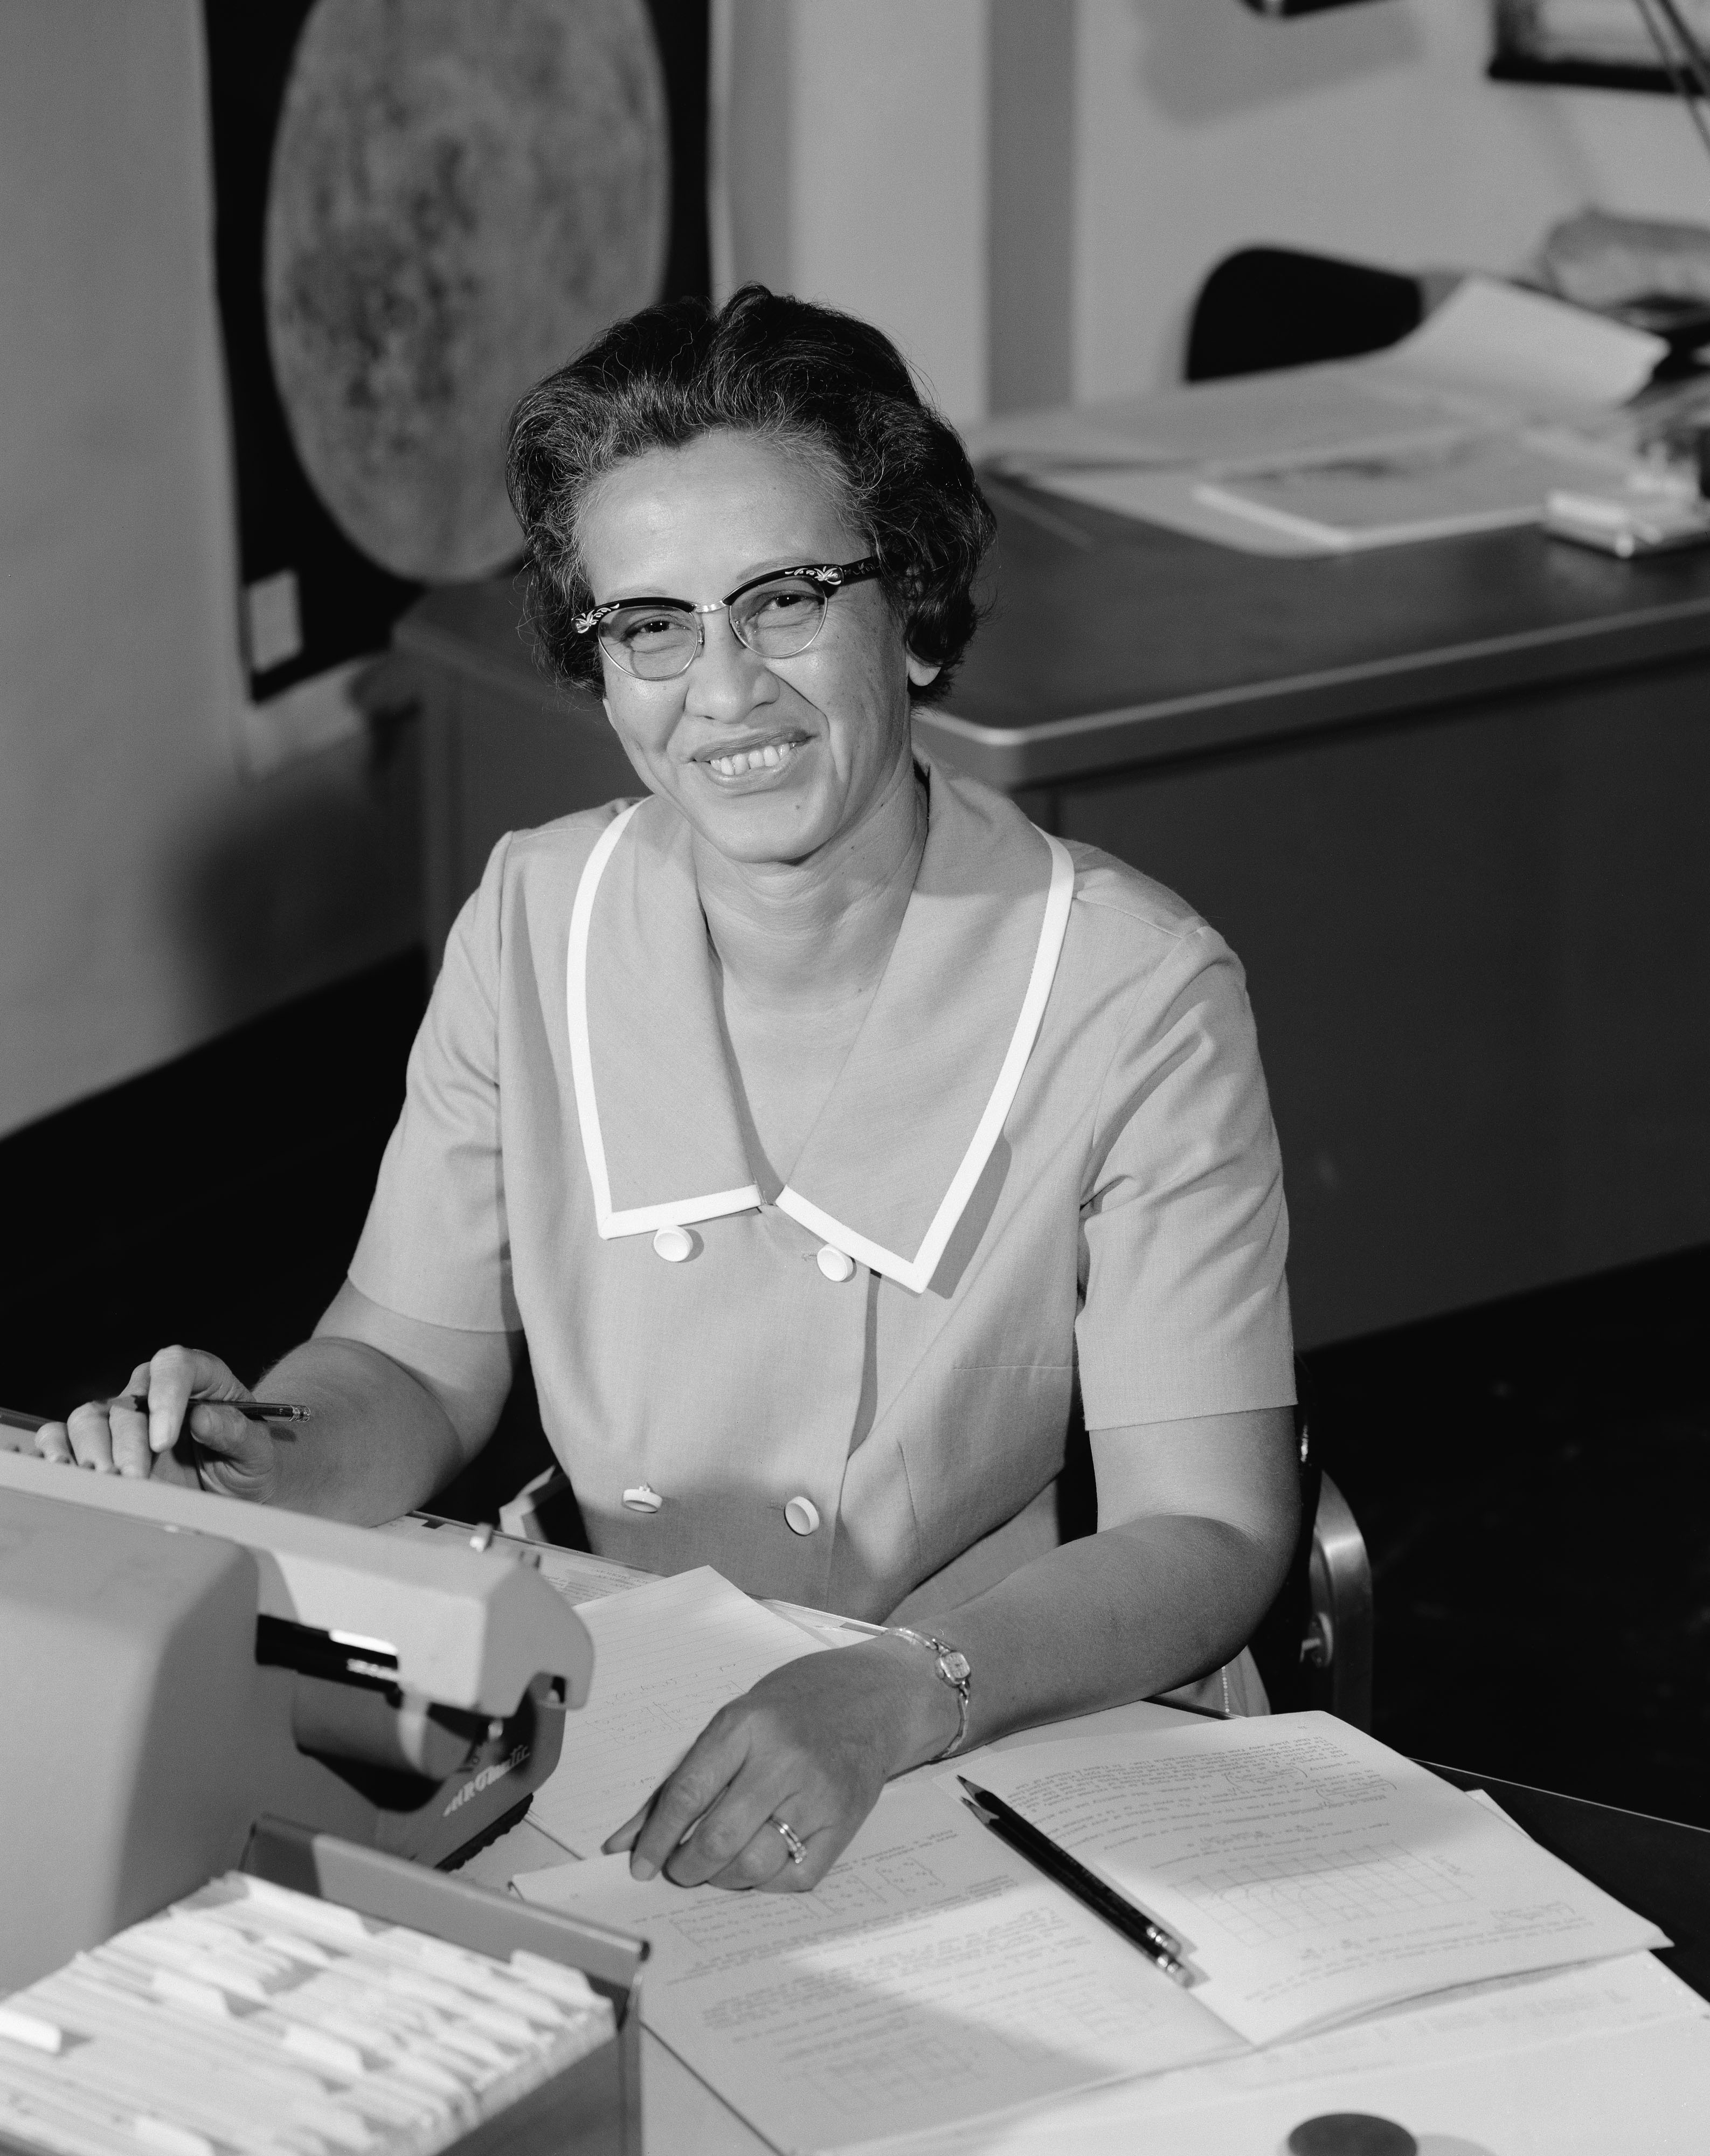
\includegraphics[width=\columnwidth]{KatherineJohnson.jpg}
%	
%	\onslide<6->{Katherine Johnson}
%\end{column}
%\end{columns}
%\onslide<7>{
%s
%}
%\end{frame}

\end{document}